\title{\vspace{160px} \textbf{\huge{Multimedia}} \\\vspace{17.5px} \LARGE{Homework 1}  \vspace{10px}}
\author{\href{https://github.com/imAlessas}{Alessandro Trigolo}}
\date{30 Aprile 2024}

\begin{document}

\maketitle\newpage

\tableofcontents
\listoffigures
\vspace{20px}
\newpage

\listoftodos\newpage


\section*{Introduzione}
Il linguaggio scelto per completare le richieste dell'homework è \texttt{Python}; all'interno del documento saranno presenti solo i punti salienti dello script, che comunque può essere ispezionato al seguente \href{https://github.com/imAlessas/computer-networks/blob/main/multimedia/hw-1/script/lossless_coding.py}{\texttt{link}}.
\todo{Inserisci introduzione dove spieghi l'obiettivo discuti brevemente come hai fatto il codice e dove trovarlo. Inserisci link a github etc}


\section{Codifica semplice} 


\vspace{15px}\subsection{Caricamento dell'immagine}
La prima richiesta dell'homework consiste nel caricare un'immagine a livelli di grigio oppure un'immagine a colori ed estrane la luminanza, approssimabile come un media tra i tre canali di colori dell'immagine. Il frammento di codice seguente incontra esattamente le richeste della prima task dove, attraverso la funzione \texttt{imread} del modulo \texttt{matplotlib.image}, l'immagine viene letta correttamente.

\begin{lstlisting}
    # Prepare to load the image
    img_file_name = "spiderman"
    img_extension = ".jpg"
    current_dir = os.getcwd()

    # path to reach the img
    path_to_img = os.path.join(current_dir, "multimedia", "hw-1", "script", "imgs") + "/"

    # loads the colored image
    gray_img = mpimg.imread(path_to_img +  img_file_name + img_extension) 

    # extracts the luminance if RGB
    if gray_img[0][0].size > 1:
        gray_img = np.dot(gray_img[..., :3], [1, 1, 1]) / 3
\end{lstlisting}

\noindent Scegliendo un'immagine a colori, in questo caso si prende come riferimento quella di \textsl{Spiderm-Man}, è quindi possibile verificare il corretto funzionamento del codice, come mostrato nella figura \ref{fig:colored-grayscale}.

\begin{figure}[h]
    \centering
    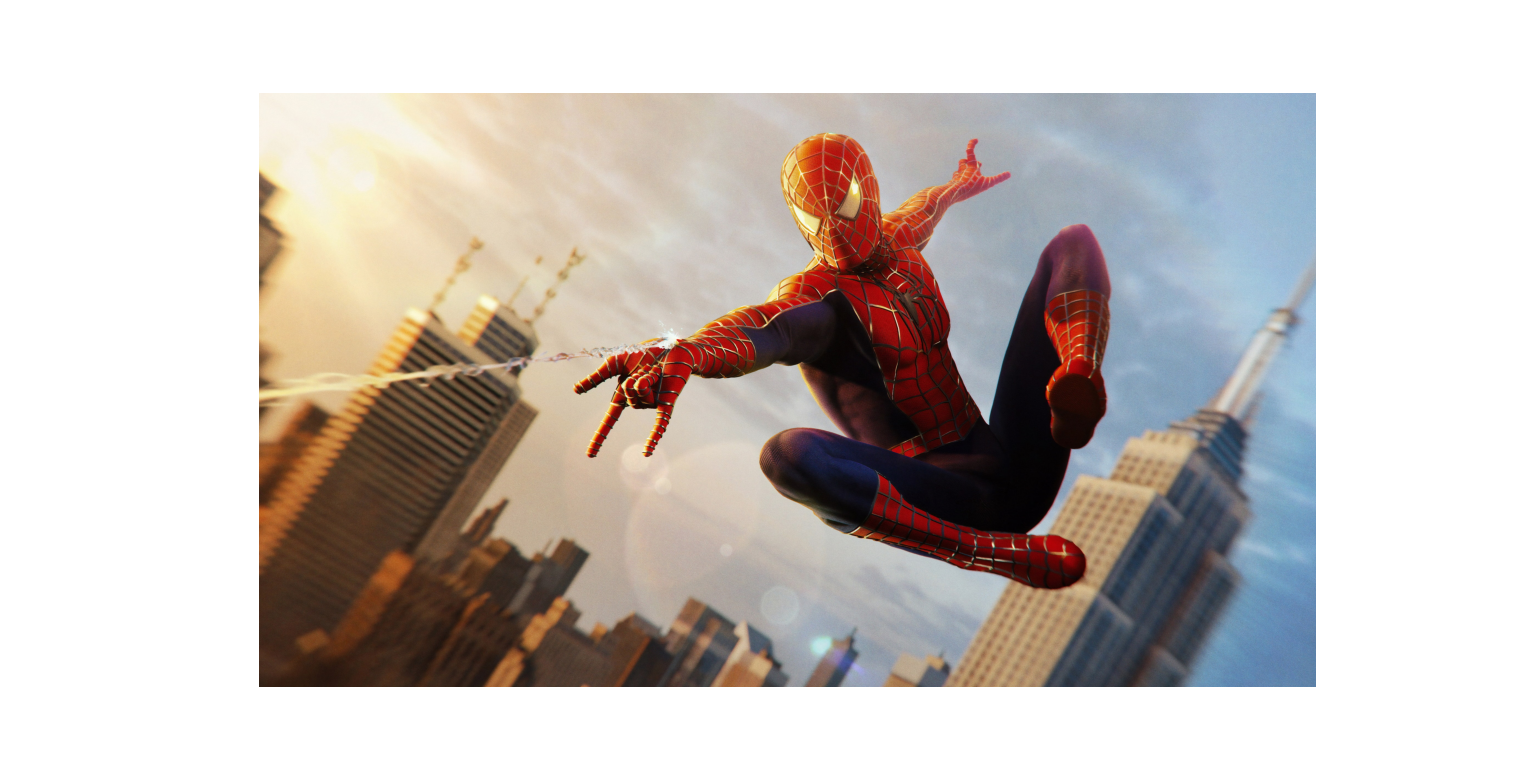
\includegraphics[width = .7\textwidth]{hw-1/report/imgs/colored.png}
    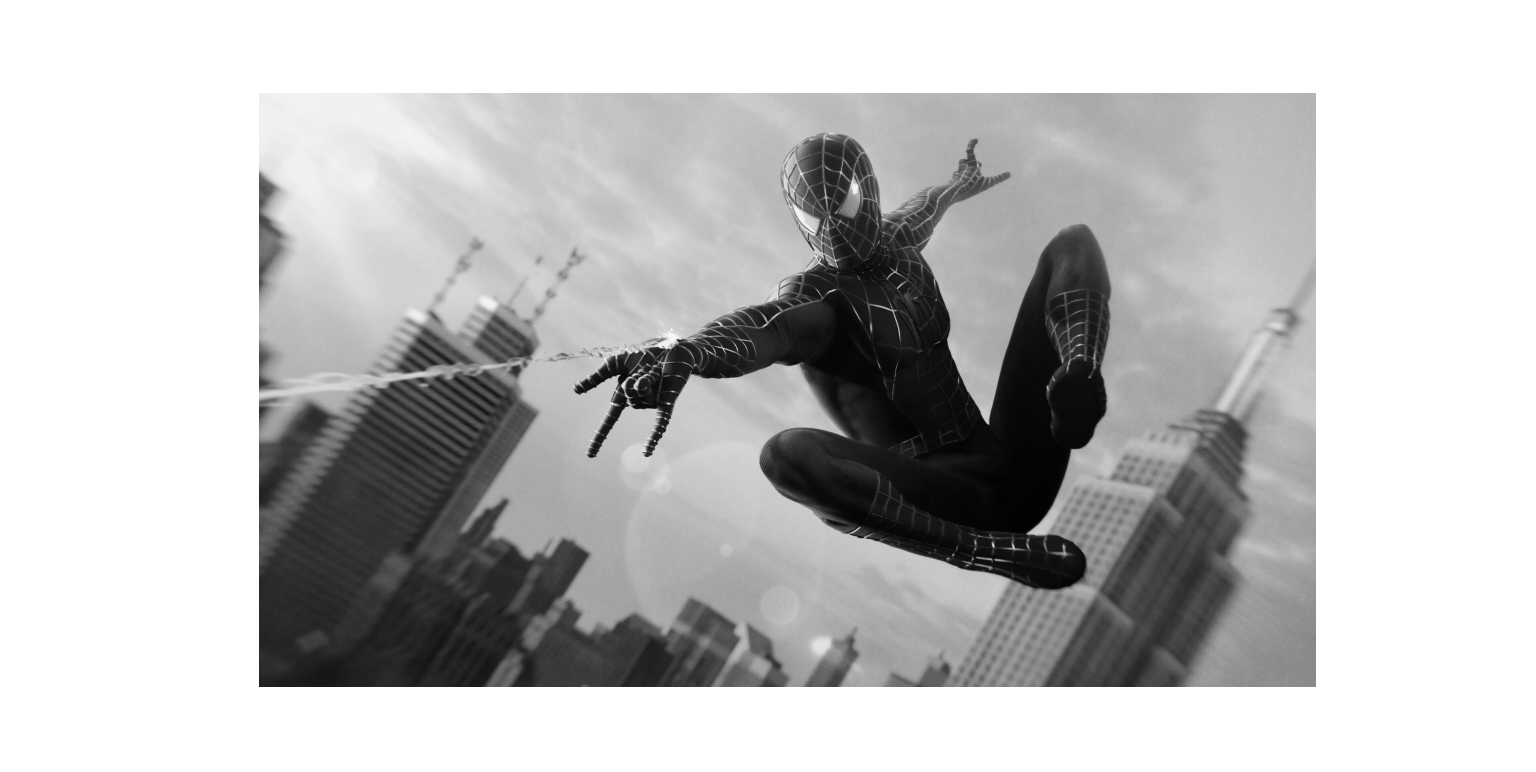
\includegraphics[width = .7\textwidth]{hw-1/report/imgs/grayscale.png}
    \caption{Estrazione della luminaza da una immagine a colori.}
    \label{fig:colored-grayscale}
\end{figure}



\subsection{Entropia dell'immagine}\label{img-entropy}
La seconda task dell'homework richiede di calcolare l'entropia dell'immagine in bianco e nero. L'entropia di una variabile aleatoria $X$ (in questo caso l'immagine) è definita come l'\textbf{informazione media} degli eventi della sorgente; l'informazione di un evento è descritta dalla funzione seguente:

\begin{gather*}
    I(X) = \log_2\left( \frac{1}{p_i} \right)
\end{gather*}

\noindent Che è una variabile che diminuisce all'aumentare della probabilità dellevento $p_i$. Questo è ragionevole in quanto più un evento è imporbabile (quindi $p_i \to 0$) e più la sua informazione è alta ($I(X) \to +\infty$). Assumendo che gli eventi della sorgente siano indipendenti, l'informazione media si traduce nella seguente formula:

\begin{gather*}
    H(X) = E[I(X)] \, = \, \sum_{i = 1}^M p_i\log_2\left( \frac{1}{p_i} \right) \, = \, - \sum_{i = 1}^M p_i\log_2{p_i}
\end{gather*}

\noindent Dove con $M$ si indica il numero di elementi nell'insieme $X$. Questa formula si riassume nel seguente script, dove la variabile contenente l'immagine in bianco e nero viene trasposta e convertita in un vettore di pixel monodimensionale. In secondo luogo attraverso la funzione \texttt{numpy.histogram} vengono contate il numero di occorrenze per ogni valore di pixel. Successivamente, per calcolare la probabilità, si divide il numero di occorrezze per il numero totale di occorrenze, escludendo eventuali valori diversi da zero. Una volta calcolare la probabilità, attraverso le funzioni  \texttt{numpy.sum} e \texttt{numpy.log2} si ottiene il valore dell'entropia $H(X)$.


\begin{lstlisting}
    # flatten the transposed matrix to read pixels row by row
    raster_scan = np.transpose(gray_img).flatten()

    # count the occurrences of each pixel value
    occurrencies = np.histogram(raster_scan, bins=range(256))[0]

    # calculate the relative frequencies
    rel_freq = occurrencies / np.sum(occurrencies)

    # remove zero-values of probability
    p = rel_freq[rel_freq > 0]

    # compute and display the entropy
    HX = np.sum(p * np.log2(1 / p))
    print(f"The entropy of {img_file_name}{img_extension} is {HX:.3f} bpp")
\end{lstlisting}

\noindent Dopo aver eseguito lo script, l'entropia dell'immagine scelta è di \textbf{7.581 bpp}.



\vspace{15px}\subsection{Codifica con dizionario}
La terza task chiede di utilizzare una compressione a dizionario, come \texttt{zip} nel caso di \textsl{Windows} per poi calcolare il \textsl{bitrate} risultante. Lo script necessario per soddisfare la richiesta è presentato nel frammento di codice sottostante. In particolare le prime righe si occupano di "zippare" il file mentre le istruzioni seguenti estraggono la dimensione dell'immagine compressa (in bytes). Infine nelle ultime linee del frammento di codice viene computato l'effettivo \textsl{bitrate} dividendo la dimensione del file compresso con la dimensione dell'immagine originale.

\begin{lstlisting}
    # change the current working directory to the directory containing the image
    os.chdir(path_to_img)

    # zip the image
    cmd = f"zip {img_file_name}.zip {img_file_name}{img_extension}"
    os.system(cmd)
    
    # get the zip bytes
    zip_bytes = os.stat(f"{img_file_name}.zip").st_size

    # get img size
    height, width = gray_img.shape
    img_size = width * height

    # get the birate
    zip_bitrate = zip_bytes * 8 / img_size 

    print(f"The bitrate of {img_file_name}.zip is {zip_bitrate:.3f} bpp")
\end{lstlisting}

\noindent Dunque, dopo aver eseguito lo script si ottiene il valore del bitrate, corrispondente a \textbf{2.657 bpp}. 



\vspace{15px}\subsection{Discussione risultati parziali}\todo{migliora risposta task 3}
Il risultato trovato calcolando il bitrate della codifica con dizionario (1.340 bpp) è molto più basso rispetto al volore dell'entropia $H(X)$, calcolato nel primo punto (7.530 bpp), suggerendo che quindi la codifica con dizionario risulta efficace nel ridurre la quantità di informazione necessaria per rappresentare i dati, sfruttando le ridondanze presenti nel segnale.




\vspace{15px}\subsection{Codifica semplice}\label{simple-coding}
La quinta richiesta dell'homework è quella di effettuare una codifica predittiva \textsl{semplice}. In particolare, data l'immagine, definita come un vettore chiamato $x(n)$, la codifica predittiva è definita come segue:

\begin{gather*}
    x(n) = 
    \begin{cases}
        128 \hspace{37px} \text{se } \, n = 0 \\
        x(n - 1) \hspace{15px} \text{altrimenti}\\
    \end{cases}
\end{gather*}

\noindent Di conseguenza l'errore di predizione $y(n)$ sull'immagine $x(n)$ è dato da:

\begin{gather*}
    y(n) = 
    \begin{cases}
        x(n) - 128 \hspace{37px} \text{se } \, n = 0 \\
        x(n) - x(n - 1) \hspace{15px} \text{altrimenti}\\
    \end{cases}
\end{gather*}

\noindent Tale codifica si traduce nel seguente codice Python, dove viene utilizzato il vettore \texttt{raster\_scan} contenete il vettore dell'immagine in scala di grigi.

\begin{lstlisting}
    # calculate prediction error
    simple_coding_error = np.concatenate(([raster_scan[0] - 128], np.diff(raster_scan.astype(float))))

    # plot error graph
    simple_coding_error_img = np.transpose(np.reshape(np.abs(simple_coding_error), (width, height)))

\end{lstlisting}

\noindent Dopo aver eseguito lo script soprastante si ottiene l'immagine mostrata nella figura \ref{fig:simple-coding}.
\begin{figure}[h]
    \centering
    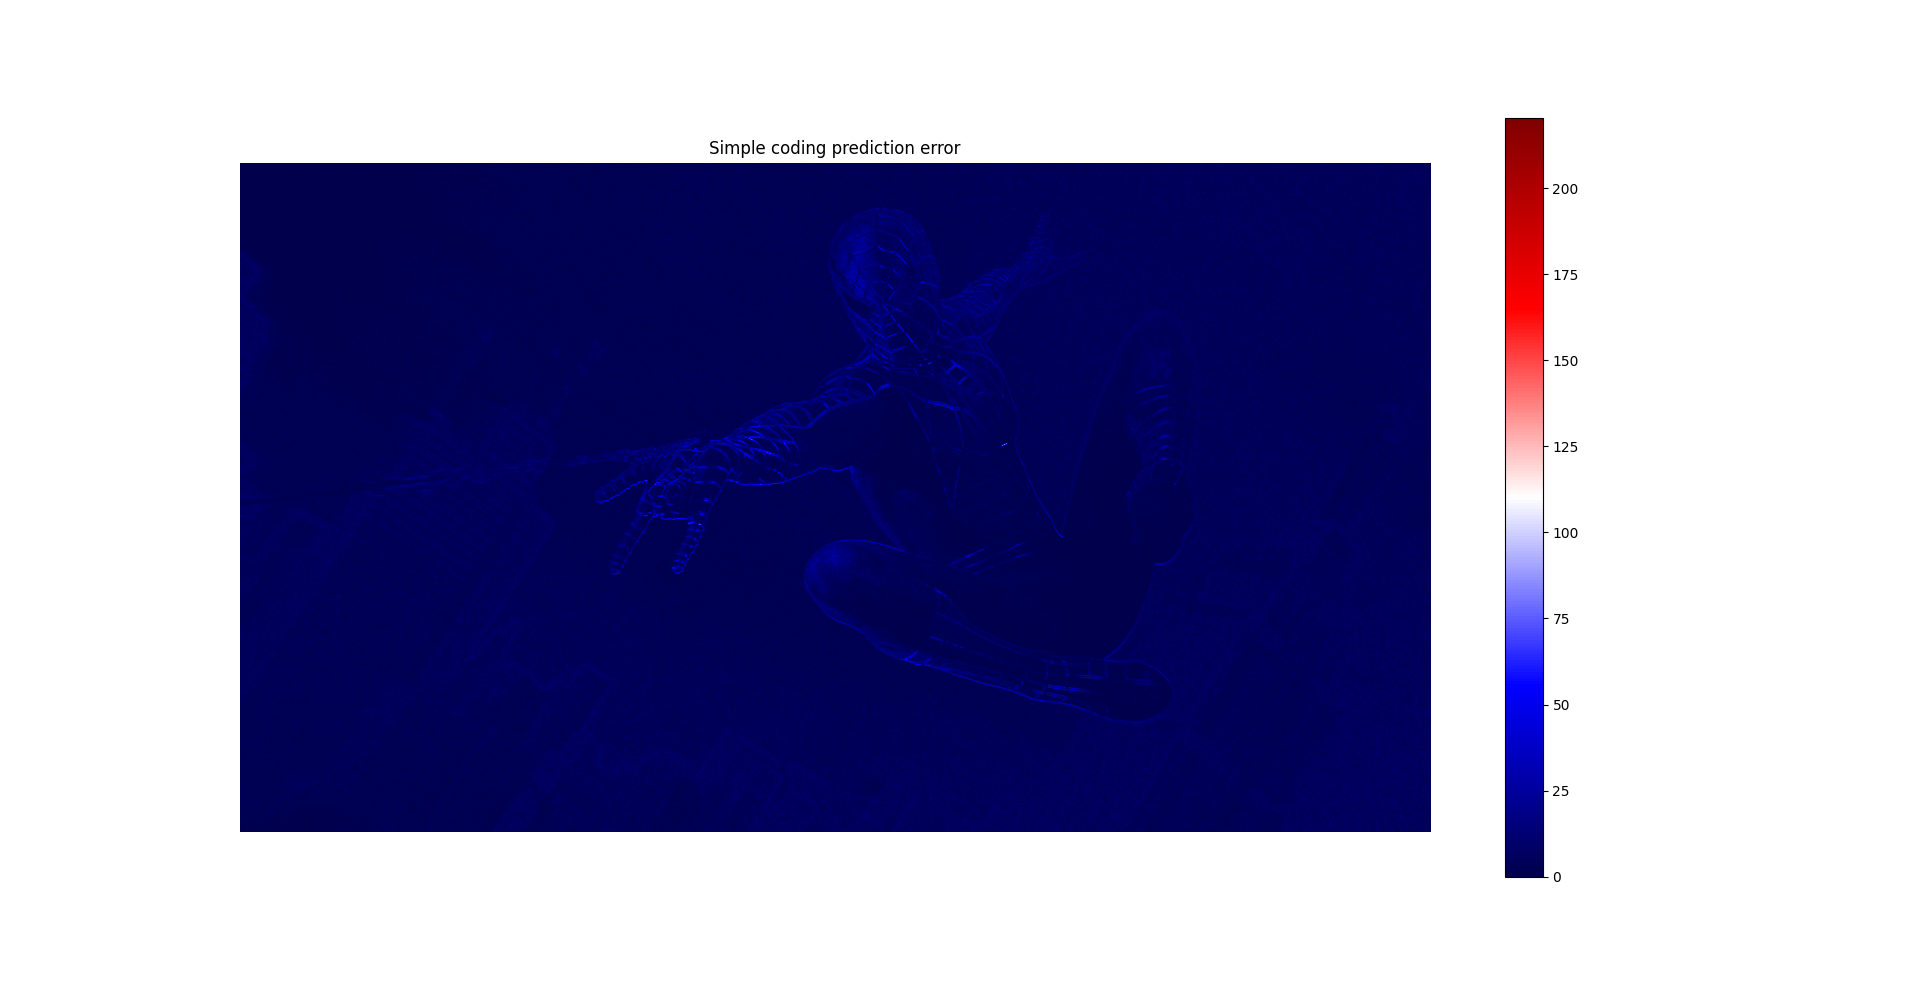
\includegraphics[width = .9\textwidth]{hw-1/report/imgs/simple-coding.png}
    \caption{Rappresentazione del modulo dell'errore di predizione nella codifica semplice.}
    \label{fig:simple-coding}
\end{figure}
Dall'immagine si può notare che le zone più chiare, ovvero le zone in cui il predittore ha fatto più errori, sono le zone dei contorni, come i contorini del personaggio raffigurato. Questo perchè la differenza dei colori tra una sezione e l'altra è particolarmente accentuata. D'altro canto, le zone colorate di blu sono le zone dove i colori sono più uniformi: eccoil quindi che i palazzi e  cielo sono per lo più dello stesso colore, suggerendo una zona dove la variazione di colore - e quindi di informazione - è molto bassa.



\subsection{Entropia dell'errore di predizione}
La richiesta seguente è quella di calculare il valore dell'entropia dell'errore di predizione $y$. Utilizzando uno script del tutto simile a quello utilizzato nella task \ref{img-entropy} possiami quindi calcolare l'entropia richiesta.

\begin{lstlisting}
    # count the occurrences of each prediction error value
    occ, _ = np.histogram(simple_coding_error, bins = range(-255, 256))

    # calculate the relative frequencies and remove any probability == 0
    freqRel = occ / np.sum(occ)
    p = freqRel[freqRel > 0]

    # calculate the entropy
    HY = np.sum(p * np.log2(1 / p))
    
    print(f"The entropy of the simple prediction error of {img_file_name} is {HY:.3f} bpp")
\end{lstlisting}

\noindent Dopo l'esecuzione dello script si ottiene che l'entropia dell'errore di predizione semplice è \textbf{4.382 bpp}.



\subsection{Exp Golomb}\label{exp-golomb}\todo{capisci cosa significa il valore EG-bpp}
Seguedo le direttive della task numero 7, calcoliamo la codifica esponenziale di Golomb (detta anche \textsl{exp-Golomb}), la quale dato un numero intero ritorna la sua codifica binaria.

Tale codifica può essere spiegata prima affrontando il caso in cui tutti i numeri da codificare siano ineri positivi e poi tale concetto si può generalizzare. La codifica di Golomb per interi positivi, detta anche \textsl{exponential Golomb unsigned}, è deifnita come segue.

\begin{gather*}
    \text{\texttt{eg\_unsigned}}(n) =
    \begin{cases}
        1 \hspace{180px} \text{se } \, n = 0 \\
        \text{zeros}\left( \left\lfloor \log_2(n + 1) \right\rfloor \right) + \text{dec2bin}(n + 1) \hspace{20px} \text{altrimenti}
    \end{cases}
\end{gather*}

\noindent A questo, dopo aver definito la codifica senza segno, la codifica con segno, detta anche \textsl{exponential Golomb signed}, è immediata:

\begin{gather*}
    \text{\texttt{eg\_signed}}(n) =
    \begin{cases}
        \text{\texttt{eg\_unsigned}}(2n - 1) \hspace{20px} \text{se } \, n > 0 \\
        \text{\texttt{eg\_unsigned}}(-2n) \hspace{28px} \text{altrimenti}
    \end{cases}
\end{gather*}

\noindent Dopo aver definito matematicamente la codifica, è possibile tradurla in due funzioni Python molto seplici, che riassumono esattamente quanto già osservato.

\begin{lstlisting}
    def exp_golomb_signed(n):
        """
        Computes the Exp-Golomb code for signed integers.
        """

        if n > 0:
            return exp_golomb_unsigned(2 * n - 1)
            
        return exp_golomb_unsigned(-2 * n)
        
    def exp_golomb_unsigned(n):
        """
        Computes the Exp-Golomb code for non-negative integers.
        """

        # handle the case where N is zero
        if n == 0:
            return '1'
        
        # returns the coded string of bits
        return '0' * int( math.floor( math.log2(n + 1) ) ) + format(n + 1, 'b')
\end{lstlisting}

\noindent Possiamo quindi ora occuparci di calcolare quanto richiesto dalla consegna. Per calcolare il numero di bit necessari utilizzando la codifica esponenziale di Golomb, è sufficiente calcolare la codifica per ogni errore della predizione semplice. La lunghezza delle codifica di ciascun valore viene sommata ottenendo quindi il numero totale di bit necessari per codificare l'errore. Infine, per ottenere il bitrate di codifica è necessario dividere il numero totali di bit per la grandezza dell'immagine. Il seguente script ricopre esattamente queste direttive.

\begin{lstlisting}
    def exp_golomb_count(vector):
        """
        Calculate the bitrate based on the exponential Golomb code for a given vector.
        """

        bit_count = 0
        for symbol in vector:
            bit_count += len(exp_golomb_signed(int(symbol)))

        return bit_count

    exp_golomb_bit = exp_golomb_count(simple_coding_error) 

    exp_golomb_bpp = exp_golomb_bit / img_size

    print(f"The number of bits for the simple coding is {exp_golomb_bit}")
    print(f"The bitrate of the simple coding is {exp_golomb_bpp:.3f}\n")
\end{lstlisting}

\noindent Dopo l'esecuzione dello script, il bitrate di codifica ha il valore di \textbf{4.980 bpp}.


\subsection{Conclusioni}
Cerchiamo ora di ottenere dei dati statistici che ci permettano di trarre delle informazioni utili. Si sono quindi prese le immagini in scala di grigi - formato \texttt{.pgm} - fornite nella demo, e si è eseguito il codice per ciascuna immagine. I risultati trovati eseguendo lo script descitto nelle precedenti sezioni per ogni immagine sono stati riassunti nella seguente tabella (\ref{tab:simple-conclusions}).


\begin{table}[h]
    \centering
    \renewcommand{\arraystretch}{1.5}
    \begin{tabular}{ | c | c c c c | }
        \hline
        \textbf{img} & \texttt{.pgm} & \texttt{.zip} & \texttt{error} & \texttt{EG-coding} \\\hline\hline

        einst & 6.785  & 6.391 & 5.343 & 6.897 \\

        house & 7.056  & 4.002 & 3.613 & 3.786 \\

        lake & 7.484  & 6.884 & 5.656 & 7.094 \\

        lena & 7.445  & 6.808 & 4.675 & 5.542 \\

        peppers & 7.594  & 7.081 & 5.026 & 6.261 \\

        plane & 6.704  & 5.714 & 4.675 & 5.252 \\

        spring & 7.157 & 6.918 & 5.342 & 6.757 \\
        \hline

    \end{tabular}
    \caption{Dati ottenute dalle varie istanze di esecuzione dello script, con immagini diverse.}
    \label{tab:simple-conclusions}
    \renewcommand{\arraystretch}{1}
\end{table}

\noindent Osservando la tebella riassuntiva si possono notare dei pattern tra i vari risultati. Prima di tutto va osservato che, ragionevolmente, l'immagine originale ha un'entropia maggiore rispetto ad una qualsisa forma di codifica o di compressione. Questo risultato suggerisce che tale ridondanza può essere sfruttata al fine di comprimere l'immagine. Osservando infatti la seconda colonna, contenete i risultati della codifica a dizionario, possiamo osservar che tali valori sono nettamente ridotti rispetto all'immagine originale; in particolare si osserva una differenza notevole nell'immagine \texttt{house}. 

In secondo luogo si osserva la differenza tra il bitrate dell'errore della codifica semplice e quello della compressione in zip. Si nota che il primo, in ciascuna iostanza di esecuzione è minore del secondo. Questo probabilmente è dovuto al fatto che la codifica predittiva riesce a comprimere meglio il file rispetto alla codifica generica. \todo{forse ho detto una cazzata}





\newpage\section{Codifica avanzata}

\vspace{15px}\subsection{Codifica avanzata}

La penultima richiesta, esige di creare un nuovo tipo di codifica, detta \textsl{avanzata} definita come segue:

\begin{gather*}
    y(n, m) = 
    \begin{cases}
        x(n, m) - 128 \hspace{161px} \text{se } \, n = m = 0 \\
        x(n, m - 1) \hspace{171px} \text{se } \, n = 0\\
        x(n - 1, m) \hspace{171px} \text{se } \, m = 0\\
        \text{med}\left[ x(n, m - 1),\, x(n - 1, m),\, x(n - 1, m - 1) \right] \hspace{15px} \text{se } \, m = \text{MAX}\\
        \text{med}\left[ x(n, m - 1),\, x(n - 1, m),\, x(n - 1, m + 1) \right] \hspace{15px} \text{altrimenti}
    \end{cases}
\end{gather*} 

\noindent Dove in questo caso l'immagine anziche essere vista come un vettore $x$ è vista come una matrice di dimensione $n \times m$. Le richieste della codifica sono tradotte in uno script contenente due cicli annidati - il primo che itera lungo le righe della matrice e il secondo che itera lungo le colonne - dove allintero sono presenti una serie di \texttt{if} statement che soddisfano la definizione di codifica avanzata precedentemente citata. Inoltre si osserva la mediana dei tre valori è calcolata tramite una funzione definita dall'utente, descritta anch'essa all'interno dello script. 

\begin{lstlisting}
# median function for advanced coding
def median(a, b, c):
    vector = [a, b, c]
    vector.remove(min(vector))
    vector.remove(max(vector))
    
    return vector[0]



# blank image 
predicted_img = np.zeros_like(gray_img)

# iterates through the rows (height)
for row in range(height):

    # iterates through the cols (width)
    for col in range(width - 1):

        if row == 0 and col == 0:   # first pixel
            predicted_img[row][col] = gray_img[row][col] - 128
        
        elif row == 1:              # first row
            predicted_img[row][col] = gray_img[row][col - 1]
        
        elif col == 1:              # first col
            predicted_img[row][col] = gray_img[row - 1][col]
        
        elif col == (width - 1):    # last col
            predicted_img[row][col] = median(gray_img[row - 1][col], gray_img[row][col - 1], gray_img[row - 1][col - 1])

        else:                       # other cases
            predicted_img[row][col] = median(gray_img[row - 1][col], gray_img[row][col - 1], gray_img[row - 1][col + 1])

adv_coding_error = gray_img - predicted_img
\end{lstlisting}

\noindent Dopo aver eseguito lo script è possibile mostrare l'errore di predizione sottraendo l'immagine predetta \texttt{predicted\_img} con l'immagine iniziale \texttt{img} e "plottando" il suo valore assoluto come segue mediante uno script simile a quello mostrato per la codifica semplice (\ref{simple-coding}). L'immagine mostrata in figura \ref{fig:advanced-coding} è ciò che risulta degli errori commessi durante la predizione.

\begin{figure}[h]
    \centering
    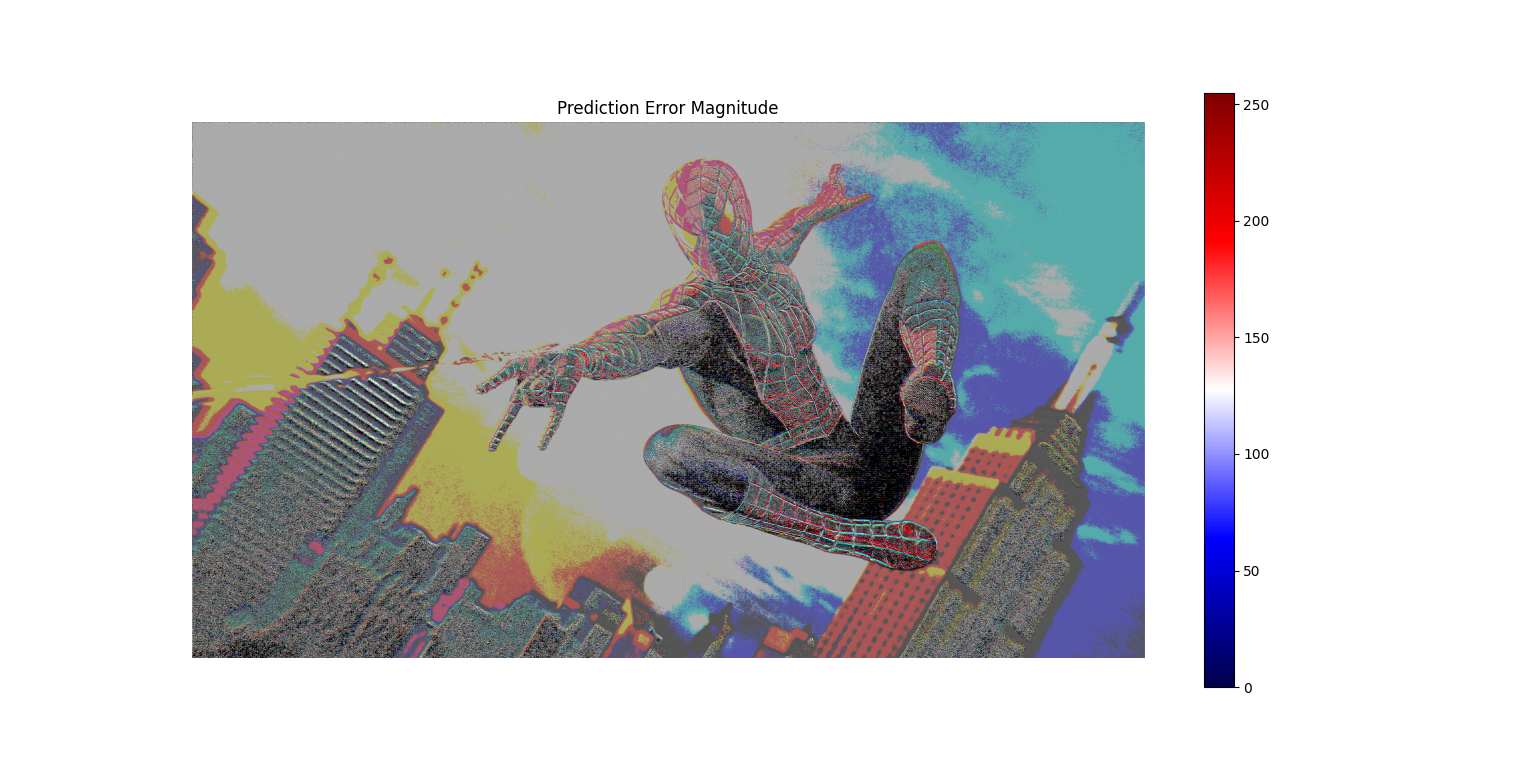
\includegraphics[width = .9\textwidth]{hw-1/report/imgs/advanced-coding.png}
    \caption{Rappresentazione del modulo dell'errore di predizione nella codifica avanzata.}
    \label{fig:advanced-coding}
\end{figure}

\FloatBarrier\noindent Si osserva che per quanto l'immagine \ref{fig:advanced-coding} sia simile alla figura \ref{fig:simple-coding}, è presente una differenza: è sufficente mostrare un'immagine che contenga la differenza in modulo tra le varaibili \texttt{adv\_coding\_error} e \texttt{simple\_coding\_error}. Dal risultato, mostrato nella figura \ref{fig:error-difference}, si può notare che non è di colore uniforme ma presenta diverse sfumature di blu, suggerendo quindi una bassa differenza tra le due che quindi le rende non identiche.

\begin{figure}[h]
    \centering
    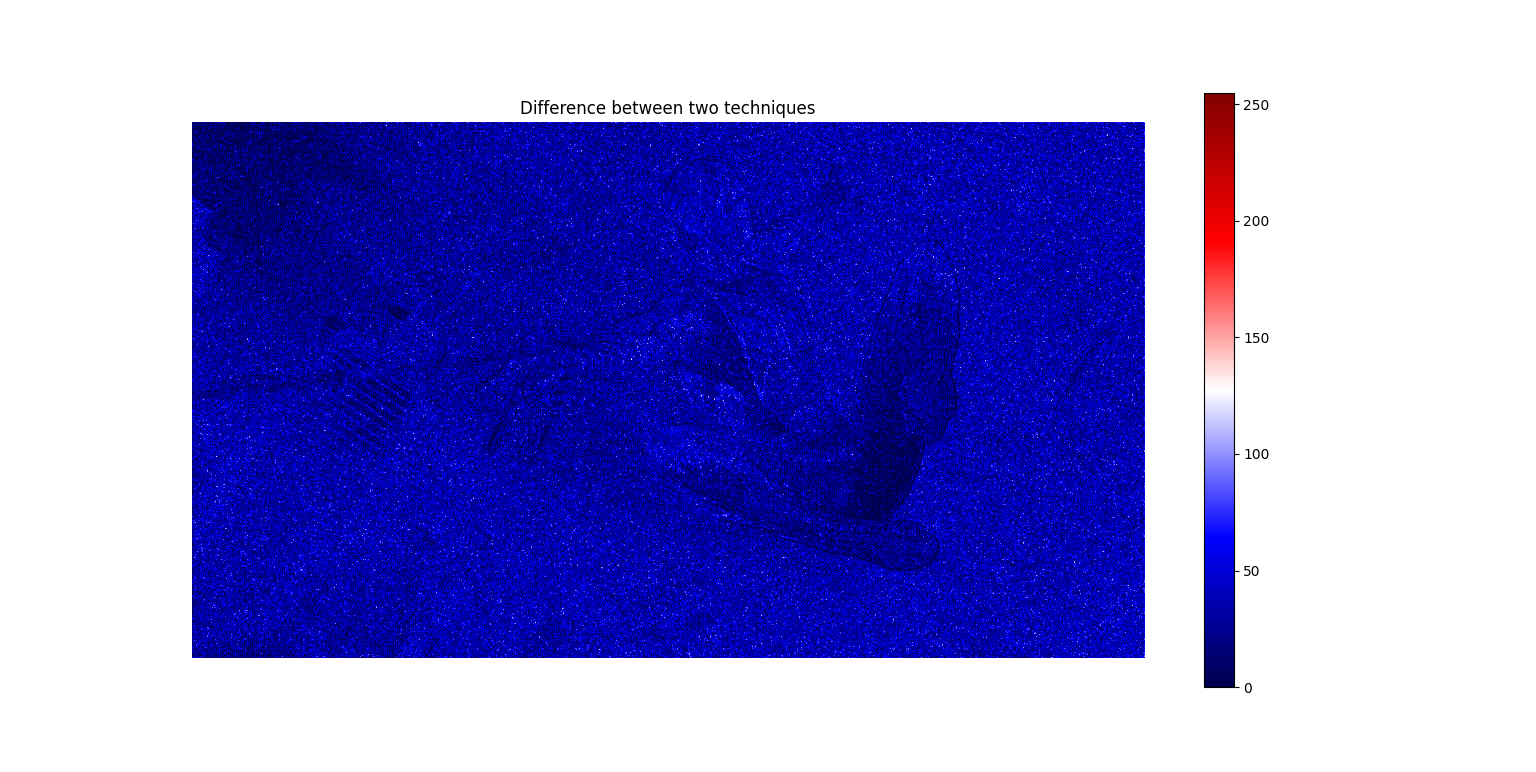
\includegraphics[width = .9\textwidth]{hw-1/report/imgs/error-difference.png}
    \caption{Rappresentazione della differenza tra l'errore della codifica semplice e della codifica avazata.}
    \label{fig:error-difference}
\end{figure}












\begin{comment}

    (1) Entropia b&w:       7.530 bpp
    (2) Bitrate .zip:       1.340 bpp
    (3) discussion
    (4) simple-coding-img
    (5) Bitrate EG:         10.0135 bpp
    (6) advanced-coding-img
    (7) Bitrate EG:         9.7443 bpp

\end{comment}

\end{document}
